\section{Обзор предметной области}
\label{sec:domain}

В данном разделе будет произведён обзор предметной области задачи, решаемой в рамках дипломного проекта; рассмотрены вопросы о сущности байесовых сетей и принципе их работы; приведена оценка сложности различных проблем, возникающих при применении вероятностных сетей для решения прикладных задач.
Также будут рассмотрены принципы работы алгоритмов вывода структуры по данным, реализованных в программном обеспечении разработанном в рамках дипломного проекта, и произведено сравнение с существующим ПО для решения схожих задач.

\subsection{Байесовы сети}
\label{sub:domain:bayes_net}
Байесовы сети являются разновидностью вероятностных графовых моделей (Probabilistic Graphical Models, PGM), представляющих вероятностные и причинно"=следственные отношения между переменными в статистическом информационном моделировании~\cite{terehov_2003}.
Вероятностные сети являются одним из возможных способов представления совместного распределения множества случайных величин.
Данный способ представления распределения является более компактным, чем хранение вероятностей для всех возможных назначений.
Здесь и далее под назначением случайных величин $ X_1, X_2, \dotsc, X_n $ понимаются определенные значения, которые принимают случайные величины, т.\,е. значения $ x_1, x_2, \dotsc, x_n $.
Табличное представление совместного распределения растет экспоненциально количеству переменных и состояний, которые эти переменные могут принимать. 
Например, чтобы задать совместное распределение $ 100 $ бинарных случайных величин необходимо запомнить $ 2^{100} - 1 $ параметр распределения, что не представляется возможным.
Помимо компактного представления функции распределения такие сети кодируют отношения безусловной и условной независимости, что является важным для понимания причинно"=следственных отношений между переменными в решаемой задаче.
Благодаря информации о независимости, распределение $ P(X_1, X_2,\dotsc, X_n) $ может быть факторизовано более просто, чем с использованием правила разложения условных вероятностей $ P(X_1, X_2,\dotsc, X_n) = P(X_1) P(X_2|X_1) \dotsm P(X_n|X_1,\dotsc,X_{n-1}) $.
Если имеется некая классическая байесова сеть, значит она кодирует информацию о независимости между переменными.
При наличии данной информации совместное распределение случайных величин может быть факторизовано по формуле:
\begin{equation}
  \label{eq:domain:bayes_net:joint_disitr}
  P(X_1, X_2,\dotsc, X_n) = \prod_{i = 0}^{n}{P(X_i|X_{\pi_i})} \text{\,,}
\end{equation}
\par
\begin{tabular}{@{}ll@{ --- }p{0.74\textwidth}}
где & $ \pi_i $ & множество индексов переменных"=родителей для переменной $X_i$.\\[\parsep]
\end{tabular}

Данное представление совместного распределения все так же имеет экспоненциальный рост количества стохастических параметров от количества переменных и их состояний.
Но на практике, обычно сети имеют небольшую связанность, далекую от полного графа, что позволяет представлять совместное распределение с помощью достижимого количества параметров.


\label{page:domain:bayes_mod}
Необходимо отметить, что существует пример успешного коммерческого применения одной из модификаций классической байесовой сети, которая имеет полиномиальный порядок роста количества параметров.
К сожалению, работы, в которых данные сети были бы формализованы и математически доказана их корректность, пока не публиковались в открытых источниках.
Отличие данной модификации от классических байесовых сетей заключается в том, что таблицы условных распределений $ P(X_k | X_{\pi_k}) $, где $k$ "--- индекс случайной величины, ассоциированные с вершинами графа и имеющими размерность $ \alpha_k \cdot \prod_{j \in \pi_k}\alpha_j $, заменяются на $ n $ таблиц меньшего размера, представляющих условные распределения $ P(X_k | X_j) $, где $ j \in \pi_k,\ k = 1,\dotsc,n $, ассоциированных с дугами графа и имеющими общую размерность $ \alpha_k \cdot \sum_{j \in \pi_k}\alpha_j $, где $\alpha_j$~--- количество значений, которые может принимать случайная величина $X_j$.
Также в данной модификации вершины графа содержат таблицы безусловного распределения $ P(X_k) $.
В связи с указанными изменениями в данной модификации используются несколько другие алгоритмы вывода статистических суждений.
Разработанная в рамках дипломного проекта библиотека кода предназначена для работы именно с такой модификацией байесовых сетей, т.\,к. различных инструментов для работы с классическими байесовыми сетями создано достаточно.
Несмотря на это, было сделано предположение, что структура классической байесовой сети и описанной выше модификации будет совпадать, и алгоритмы построения, применимые для нахождения структуры по данным для классической байесовой сети, подойдут для указанной модификации.
Следовательно, сама библиотека может быть использована и для вывода структуры классических сетей, что будет неоднократно использовано далее для оценки качества структуры сети, полученной по экспериментальным данным.

Таким образом можно выделить следующие понятия и компоненты, из которых состоят вероятностные сети~\cite{terehov_2003}:
\begin{itemize}
  \item множество случайных переменных и направленных связей между переменными;
  \item каждая переменная может принимать одно из конечного множества взаимоисключающих значений;
  \item переменные вместе со связями образуют ориентированный граф без циклов;
  \item каждой переменной"=потомку $X_k$ с переменными"=предками $\pi_k$
приписывается таблица условных вероятностей $P(X_k | X_{\pi_k})$, либо, для вышеупомянутой модификации "--- каждой дуге между переменными $ X $ и $ Y $ сопоставляется таблица условного распределения $ P (X | Y)$, каждой вершине "--- таблица безусловного распределения $ P(X) $.
\end{itemize}

%Что такое байесовы сети (2 стр)

\subsection{Построение вероятностной сети}
\label{sub:domain:learning_structure}
Одним из первых этапов применения байесовых сетей для решения практической задачи, после формулирования проблемы в терминах вероятностей и выделения целевых переменных, является этап описания отношений <<причина"=следствие>> между переменными в виде ориентированных ребер графа~\cite{terehov_2003}.
Задание подобных отношений определяет структуру графа вероятностной сети.

От правильности выбора структуры сети зависят многие важные качественные показатели сети, такие как количество необходимых параметров, сложность вывода статистических суждений, возможность обоснования поведения сети при изменении назначений некоторых из переменных.

Исторически одним из первых способов создания байесовых сетей было привлечение экспертов в предметной области решаемой проблемы.
Построенная сеть отражала субъективное представление экспертов о проблеме и потенциально могла отличаться от истины.
Параметры условных распределений в вершинах графа отражали байесовы вероятности по мнению экспертов.
Здесь и далее под байесовой вероятностью понимается степень уверенности в истинности суждения определенного индивидуума, в отличие от частотной вероятности, которая определяется как относительная частота возникновения события в большом числе испытаний.

Далее будет рассмотрен пример ручного построения классической байесовой сети по имеющимся априорным данным о проблеме.

%О важности вывода структуры (1 стр)

\subsection{<<Ручное>> построение структуры на основе экспертных знаний}
\label{sub:domain:manual_structure}
Рассматриваемый здесь пример был взят из домашнего задания, предлагаемого в онлайн курсе Стэндфордского университета по вероятностным графовым моделям~\cite{pgm_course}.
Ниже приводится один из возможных вариантов его решения.

Необходимо разработать модель для  прогнозирования своевременности выплат клиентом задолженности банку по кредиту и другим займовым операциям, т.\,е. модель для оценки кредитоспособности клиента банка.
Банк имеет доступ к некоторой информации о клиенте, такой как его \emph{доходы} (Income), \emph{история платежей} (PaymentHistory), накопленные \emph{богатства} (Assets), \emph{возраст} клиента (Age), а также к \emph{соотношению долгов к доходам} (DebtIncomeRatio).
Банковский эксперт полагает, что целевая переменная "--- \emph{кредитоспособность} (CreditWorthiness) "--- в конечном итоге зависит от \emph{надежности} (Reliability) клиента, его прогнозируемых \emph{будущих доходов} (FutureIncome) и \emph{соотношения долгов к доходам}.
По известным на данный момент данным можно построить скелет будущей вероятностной сети "--- её структуру.
Для полноты картины создания сети вручную пример продолжается и добавляется дополнительная информация, имеющаяся у банка, которая поможет задать вероятности в таблицах условного распределения.
Необходимо отметить, что указанные вероятности будут байесовыми, т.\,к. отражают субъективное представление о поведении модели:
\begin{itemize}
  \item чем лучше история платежей клиента, тем с большей вероятностью он надежен;
  \item чем старше клиент, тем с большей вероятностью он надежен;
  \item у старших клиентов с большей вероятностью будет отличная история платежей;
  \item клиенты с высоким соотношением долгов к доходам с большей вероятностью имеют финансовые трудности, следовательно с меньшей вероятностью имеют хорошую историю платежей;
  \item чем выше доход человека, тем больше вероятность что он имеет много накопленных богатств;
  \item чем больше накопленных богатств и выше доходы клиента, тем лучше прогнозируемые будущие доходы;
  \item при прочих равных, надежные люди с большей вероятностью кредитоспособны, чем ненадежные. Также люди с более высокими прогнозируемыми доходами или с низким соотношением долгов к доходам более кредитоспособны и наоборот. 
\end{itemize}

С учетом всех приведенных выше дополнительных наблюдений, имеющихся у банка, можно сконструировать сеть и задать байесовы вероятности в таблицах распределения.
Одна из возможных структур сети приведена на рисунке~\ref{fig:domain:manual_structure:credit_net}.
Перевод условных обозначений, используемых на рисунке, на русский язык приведен ранее в тексте данного подраздела.
Таблицы с условными и безусловными вероятностями здесь не приводятся для экономии места.

Таким образом, чтобы построить классическую байесову сеть понадобилось ознакомиться с предметной областью и проконсультироваться с экспертом. 
Также необходимо было учесть все наблюдения, сделанные экспертом, и учесть его опыт и представление о предметной области.
В итоге была построена модель, которая соответствует представлению о проблеме эксперта, но на самом деле может отличаться от истинной модели проблемы.

\begin{figure}[ht]
\centering
  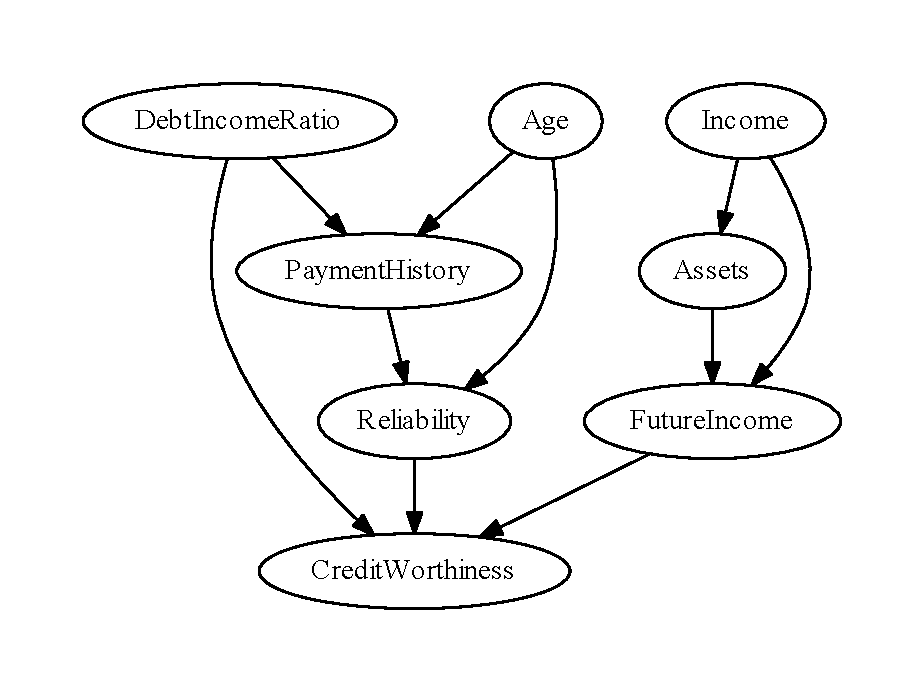
\includegraphics[scale=1]{Credit_net.pdf}  
  \caption{ Байесова сеть для оценки кредитоспособности. }
  \label{fig:domain:manual_structure:credit_net}
\end{figure}

% 2 стр

\subsection{Сложность нахождения структуры по данным}
\label{sub:domain:learning_complexity}

В предыдущем подразделе был приведен пример построения классической байесовой сети <<вручную>> с использованием экспертных знаний.
Для большинства возникающих задач можно собрать большой объём экспериментальных данных без каких"=либо усилий.
В данной ситуации возникает интересная задача "--- как построить вероятностную сеть используя лишь эти данные, прибегнув к минимуму экспертных знаний?
Данный вопрос затрагивался во многих научных работах~\cite{Lam94learningbayesian,Suzuki93,Cooper1991,terentyev_2006} и имеет различные подходы к решению, но сама задача является $\mathcal{NP}$-полной~\cite{Chickering96learningbayesian} и требует применения различных ухищрений и эвристик для автоматического построения структуры сети на практике.

Сложность задачи обоснована тем, что количество всевозможных назначений растет экспоненциально количеству переменных и их состояний.
Различные алгоритмы построения сетей используют различные оценочные метрики качества сети.
Эти метрики, обычно, включают себя подсчёт маргинализованных распределений некоторого подмножества случайных величин.
Вычисление данных распределений подразумевает подсчет суммы вероятностей экспоненциального числа назначений.
На практике во избежание большого количества вычислений используются различные приближенные методы, зависящие от метрики.
Даже при наличии возможности вычислить функцию для оценки качества сети быстро, все равно остаётся проблема супер"=экспоненциального роста количества моделей в зависимости от числа переменных.
Робинсон в работе~\cite{robinson_1977} предложил следующее рекуррентное соотношение для подсчета числа ацикличных моделей:
\begin{equation}
  r (n) =
  \begin{cases}
      1 &, n = 0 \\
      \sum_{i = 1}^{n} (-1)^{i+1} \binom{n}{i} 2^{i(n-i)} r(n - i) &, n > 0 
  \end{cases} % = n ^{2^{\mathcal{O}(n)}}
\end{equation}

Для убедительности приведем в таблице~\ref{table:domain:learning:number_of_models} некоторые числа, касающиеся количества возможных моделей для сети из $n$ переменных~\cite{terentyev_2006}.
Как видно из таблицы, для более семи вершин полный перебор выполнить проблематично.

\begin{table}[ht]
\caption{Зависимость числа моделей без циклов от количества вершин, которые нужно проанализировать при полном переборе моделей}
\label{table:domain:learning:number_of_models}
\centering
  \begin{tabular}{| >{\centering}m{0.1\textwidth} 
                  | >{\raggedleft}m{0.345\textwidth} 
                  | >{\centering}m{0.1\textwidth} 
                  | >{\raggedleft\arraybackslash}m{0.345\textwidth}|}
  \hline Число вершин & \begin{center} Моделей без циклов \end{center} & Число вершин & \begin{center} Моделей без циклов \end{center} \\
  \hline \num{1} & \num{1} & \num{6} & \num{3781503} \\
  \hline \num{2} & \num{3} & \num{7} & \num{1138779265} \\
  \hline \num{3} & \num{25} & \num{8} & \num{783702329343} \\
  \hline \num{4} & \num{543} & \num{9} & \num{1213442454842881} \\
  \hline \num{5} & \num{29281} & \num{10} & \num{4175098976430598100} \\
  \hline
  \end{tabular}
\end{table}

%Указание что это NP трудная задача (0.5)
%Табличка с оценкой количества сетей в зависимости от числа переменных (для устрашения) (0.2)

\subsection{Принцип минимальной длинны описания}
\label{sub:domain:mdl_principle}
В данном подразделе рассматривается принцип минимальной длинны описания\footnote{В англоязычной литературе используется термин minimum description length или сокращенно MDL.} (МДО) и его применимость для задания функции оценки качества обучаемой сети.
Данный принцип позволяет среди множества моделей выбрать модель с оптимальным соотношением сложности и соответствием модели наблюдаемым данным. 
Т.\,е. данный принцип позволяет выбрать несложную и <<полезную>> модель, устойчивую к проблеме переобучения\footnote{В англоязычной литературе данная проблема называется overfitting и подразумевает, что модель слишком хорошо объясняет данные на которых она обучалась, но из-за этого непригодна для прогнозирования "--- работе на данных ранее не известных.}.
Принцип МДО в своей нестрогой и наиболее общей формулировке гласит: среди множества моделей следует выбрать ту, которая позволяет описать данные наиболее коротко, без потери информации~\cite{Grunwald05atutorial}.
В контексте поиска модели байесовой сети, соответствующей экспериментальным данным, принцип МДО гласит, что нужно выбрать модель, которая минимизирует сумму длин кодирования самой модели и кодирования экспериментальных данных с помощью этой модели~\cite{Lam94learningbayesian}, что выражается формулой:
\begin{equation}
  \label{eq:domain:mdl:description_length}
  l(x^{R}[n]) = \min_{g \in G}\left[ l_{G}(g) + l_{g}(x^{R}[n]) \right] \text{\,,}
\end{equation}
\par
\begin{tabular}{@{}ll@{ --- }p{0.68\textwidth}}
где & $ x^R $ & вектор размерностью $R$, содержащий значения переменных (аттрибутов). Представлен как $ x^R =\newline= (x^{(1)}, x^{(2)}, \dotsc, x^{(R)} ) $, где атрибут $ x^{(j)} $ может принимать $ \alpha_{j} $ значений, $ j = 1,\dotsc,R.$ \\
    & $ n $ & количество случаев в экспериментальных данных;  \\
    & $ x^R[n] $ & набор экспериментальны данных; \\
    & $ G $ & множество моделей; \\
    & $ l_{G}(g) $ & длина описания модели; \\
    & $ l_{g}(x^{R}[n]) $ & длина представления данных $ x^R[n] $ моделью $ g \in G $. \\[\parsep]
\end{tabular}

Для вычисления длинны кодирования модели и длинны кодирования данных с использованием модели в реализации дипломного проекта использовались результаты, приведенные в работах~\cite{Suzuki93,terentyev_2006}.
Собственно модель вероятностной сети состоит из таблиц условных и безусловных распределений и отношений <<родитель"=потомок>> между вершинами.
Для вычисления длины кодирования модели можно воспользоваться формулой~(\ref{eq:domain:mdl:model_length}):
\begin{equation}
  \label{eq:domain:mdl:model_length}
  l_{G}(g) = \frac{\log{n}}{2} \cdot \sum_{k = 1}^{R} S_k(g) (\alpha_k - 1) \text{\,,}
\end{equation}
\par
\begin{tabular}{@{}ll@{ --- }p{0.73\textwidth}}
где & $ S_k(g) $ & количество возможных назначений переменных"=родителей переменной $X_k$, способ вычисления данного значения отличается у классических сетей и модификации упомянутой в разделе~\ref{sub:domain:bayes_net} на странице~\pageref{page:domain:bayes_mod}. \\[\parsep]
\end{tabular}

Значение функции $S_k(g)$ для классических байесовых сетей вычисляется по формуле~(\ref{eq:domain:mdl:classic_parent_states}), для модификации упомянутой в разделе~\ref{sub:domain:bayes_net} на странице~\pageref{page:domain:bayes_mod} "--- по формуле~(\ref{eq:domain:mdl:mod_parent_states}):
\begin{align}
  \label{eq:domain:mdl:classic_parent_states}
  S_k(g) &= \prod_{j \in \pi_k}\alpha_j \text{\,,} \\
  \label{eq:domain:mdl:mod_parent_states}
  S_k(g) &= \sum_{j \in \pi_k}\alpha_j \text{\,.}
\end{align}

Длинна представления данных $ l_{g}(x^{R}[n]) $ вычисляется как эмпирическая энтропия $ n $ экспериментальных наблюдений $ x^{R}[n] $ при заданной модели $ g $.
Эмпирическая энтропия может быть вычислена по формуле~(\ref{eq:domain:mdl:data_entrophy}):
\begin{equation}
  \label{eq:domain:mdl:data_entrophy}
  \mathcal{H}(x^{R}[n] | g) = 
    \sum_{k = 1}^{R}
    \sum_{s = 1}^{S_{k}(g)}
    \sum_{q = 0}^{\alpha_{k + 1} - 1}
    -n[q, s, k, g] \log \frac{n[q, s, k, g]}{n[s, k, g]} \text{\,,}
\end{equation}
\par
\begin{tabular}{@{}ll@{ --- }p{0.66\textwidth}}
где & $ n[s, k, g] $ & количество случаев в экспериментальных данных $ x^R[n] $ в которых переменные"=родители переменной $X_k$ принимают назначение $s$; \\
    & $ n[q, s, k, g] $ & количество случаев в экспериментальных данных $ x^R[n] $ в которых переменные"=родители переменной $X_k$ принимают назначение $s$, а переменная $X_k$ принимает назначение $q$. \\[\parsep]
\end{tabular}

Таким образом, приведенные выше формулы, могут быть использованы для оценки качества структуры сети и её сложности.
Имея данную оценку можно использовать различные стратегии поиска в пространстве возможных моделей, минимизируя целевую функцию~(\ref{eq:domain:mdl:description_length}).
Более подробно об используемых стратегиях поиска говорится в разделе~\ref{sec:arch_and_mod}.
За доказательствами и более подробными сведениями о применении принципа МДО в построении байесовых сетей можно обратиться к работам~\cite{Lam94learningbayesian,Suzuki93,terentyev_2006,Grunwald05atutorial}.

% MDL (2-3)


\subsection{Оценка структуры сети на основе апостериорной вероятности}
\label{sub:domain:k2_algo}
Существуют подходы, использующие байесов метод для оценки качества полученной структуры и алгоритмы на их базе пытаются максимизировать апостериорную вероятность структуры для данного набора экспериментальны данных.
Один из возможных подходов к оценке качества двух структур приведет в работе~\cite{Cooper1991}.
В программном обеспечении, разработанном в данном дипломном проекте, использовался критерий оценки качества структуры, приведенный в упомянутой выше работе.

Введем некоторые обозначения, в дополнение к тем, которые были введены в подразделе~\ref{sub:domain:mdl_principle}.
Пусть структура вероятностной сети обозначается символом $B_S$, таблицы условных распределений, ассоциированные с сетью, "--- $B_P$.
Две вероятностные сети для данного набора экспериментальных данных можно оценить по отношению~(\ref{eq:domain:k2:nets_ratio}) апостериорных вероятностей:
\begin{equation}
  \label{eq:domain:k2:nets_ratio}
  \frac{P(B_{S_i} | x^R[n])}{P(B_{S_j} | x^R[n])} =
    \frac{ \frac{P(B_{S_i}, x^R[n])}{P(x^R[n])} }
         { \frac{P(B_{S_j}, x^R[n])}{P(x^R[n])} } =
    \frac{ P(B_{S_i}, x^R[n]) }
         { P(B_{S_j}, x^R[n]) } \text{\,.}
\end{equation}

Как видно из приведенной формулы~(\ref{eq:domain:k2:nets_ratio}), научившись вычислять отношение совместных распределений, можно сравнивать апостериорные вероятности структур.
Т.\,к. в разработанном ПО использовались результаты, приведенные в работе~\cite{Cooper1991}, то считаем целесообразным привести в данном подразделе базовые формулы и предположения из вышеупомянутой работы.

Для вычисления $P(B_S, D)$ важно сделать несколько важных предположений:

\begin{itemize}
  \item 
  Экспериментальные данные содержат только дискретные случайные величины и все эти случайные величины присутствуют в истинной структуре $B_S$ модели из которой были получены эти экспериментальные данные.
  Из данного предположения следует формула~(\ref{eq:domain:k2:assumption1}):
  \begin{equation}
    \label{eq:domain:k2:assumption1}
    \int_{B_P} P(x^R[n] | B_S, B_P) f(B_P | B_S) P(B_S) dB_p \text{\,,}
  \end{equation}
  \par\hspace{\fivecharsapprox} % абзацный отступ
  \begin{tabular}{@{}ll@{ --- }p{0.74\textwidth}}
  где & $ B_P $ & вектор, содержащий значения условных вероятностей для назначений переменных из структуры $ B_S $; \\
      & $ f $ & условная плотность распределения $B_P$ при условии структуры $B_S$. \\[\parsep]
  \end{tabular}

  \item
  Случаи, зафиксированные в экспериментальных данных, независимы друг от друга, при условии зафиксированной модели, т.\,е. данное предположение подразумевает, что модель, генерирующая экспериментальные данные не меняется.
  Это предположение позволяет упростить формулу~(\ref{eq:domain:k2:assumption1}) и привести её к виду:
  \begin{equation}
    \label{eq:domain:k2:assumption2}
    P(B_S, x^R[n]) =
      P(B_S) \int_{B_P} \left[ \prod_{j = 1}^{n} P(x^R_j | B_S, B_P) \right] f(B_P | B_S) dB_P \text{\,.}
  \end{equation}

  \item
  Экспериментальные данные не должны содержать пропущенных значений для переменных из структуры $B_S$. 
  Введем дополнительные обозначения.
  Пусть $x_j^{(i)}$ представляет значение $i$-й переменной в $j$-м случае.
  Пусть $\phi_i$ представляет из себя вектор уникальных назначений переменных"=родителей для $i$-й переменной, т.\,е. вектор уникальных назначений для $ \forall X_k,\ k \in \pi_i$.
  Пусть $\sigma(i, j)$ индексная функция, которая возвращает индекс назначения $\pi_i$ в $j$-ом случае из вектора $\phi_i$.
  Введем обозначение для длинны вектора $q_i = | \phi_i |$.
  Теперь с учетом предположения об отсутствии пропущенных значений можно вычислить вероятность конкретного случая из экспериментальных данных по формуле:
  \begin{equation}
    \label{eq:domain:k2:case_prob}
    P(x^R_j | B_S, B_P) = 
      \prod_{i = 1}^{R} = P(X_i = x_j^{(i)} | \phi_i[\sigma(i, j)], B_P) \text{\,.}
  \end{equation}
  Подставляя выражение~(\ref{eq:domain:k2:case_prob}) в формулу~(\ref{eq:domain:k2:assumption2}) получим:
  \begin{align}
    \label{eq:domain:k2:assumption3}
    P(B_S, x^R[n]) =
      P(B_S)
      \int_{B_P}\left[ \prod_{j = 1}^{n}\prod_{i = 1}^{R} P(X_i = x_j^{(i)} | \phi_i[\sigma(i, j)], B_P)  \right] &\times \notag\\ 
      \times f(B_P | B_S) dB_P \text{\,.}
  \end{align}
  Пусть для выбранных $i$ и $j$ $f(P(x_i | \phi_i[j], B_P))$ обозначает плотность распределения возможных значений $P(x_i | \phi_i[j], B_P)$.
  Необходимо сделать еще одно предположение.

  \item Для $ 1 \le i, i' \le n$, $ 1 \le j \le q_i $, $1 \le j' \le q_i $, если 
  $ij \neq i'j'$, то распределение $f(P(x_i | \phi_i[j]))$ не зависимо от распределения $f(P(x_{i'} | \phi_{i'}[{j'}]))$.
  Данное предположение по свой сути полагает, что до того, как были получены экспериментальные данные, все возможные назначения равновероятны.
\end{itemize}

С учетом приведенных выше предположений и теоремы, приведённой и доказанной в работе~\cite{Cooper1991}, можно привести формулу для вычисления $P(B_S, D)$:
\begin{equation}
  \label{eq:domain:k2:model_and_data_prob}
  P(B_S, x^R[n]) = 
    P(B_S)
    \prod_{i = 1}^{R}
    \prod_{j = 1}^{q_i}
    \frac{(\alpha_i - 1)!}
         {(n[\phi_i[j], i, B_S] + \alpha_i - 1)!}
    \prod_{k = 1}^{\alpha_i}
      n[v_{ik}, \phi_i[j], i, B_S]! \text{\,,}
\end{equation}
\par
\begin{tabular}{@{}ll@{ --- }p{0.74\textwidth}}
где & $ v_{ik} $ & $k$-е возможное назначение переменной $X_i$. \\[\parsep]
\end{tabular}

Формула~(\ref{eq:domain:k2:model_and_data_prob}) позволяет вычислить значение $P(B_S, x^R[n])$, если известна вероятность $P(B_S)$ и подсчитана оставшаяся часть формулы на основе экспериментальны данных $x^R[n]$.
Но из-за того, что $P(B_S)$ является чаще неизвестной величиной, чем известной, предполагают, что все возможные структуры сети равновероятны и $P(B_S)$ является некой малой константой.
Апостериорную вероятность структуры, при условии данных можно вычислить по формуле:
\begin{equation}
  \label{eq:domain:k2:aposteriori_structure_given_data}
  P(B_S | x^R[n]) = 
    \frac{P(B_S, x^R[n])}
         {\sum_{B_S}P(B_S, x^R[n])} \text{\,.}
\end{equation}

Но, как уже упоминалось, множество возможных структур слишком велико, и на практике значение апостериорной вероятности можно вычислить лишь для малых сетей либо приблизительно. 
В разделе~\ref{sec:arch_and_mod} будет более подробно рассмотрена модификация оценки апостериорной вероятности~(\ref{eq:domain:k2:model_and_data_prob}), применимая на практике.

%Оценка апостериорных вероятностей (K2) (2-3)

\subsection{Общая структура алгоритмов}
\label{sub:domain:other_algos}
В предыдущих двух подразделах были рассмотрены два подхода к оценке качества структуры сети при известных экспериментальных данных.
Как уже упоминалось ранее, выбор функции оценки сети является лишь одним из компонентов большинства алгоритмов построения структуры сети по данным.
Важной частью алгоритма является также выбор стратегии поиска в пространстве возможных структур.
От выбора стратегии поиска зависит трудоемкость алгоритма, качество найденной сети и, собственно, её структура.
В ПО разработанном в рамках дипломного проекта реализовано несколько различных алгоритмов нахождения структуры на основе оценки апостериорной вероятности из подраздела~\ref{sub:domain:k2_algo} и оценки на основе принципа МДО из подраздела~\ref{sub:domain:mdl_principle}.
Стоит упомянуть, что в разработанном ПО реализованы разные стратегии поиска для разных оценок. 
Так алгоритмы использующие оценку МДО могут находить сети произвольной структуры без каких-либо априорных знаний о предметной области.
С другой стороны, для уменьшения пространства возможных решений, алгоритм, использующий оценку апостериорной вероятности, требует априорных знаний об упорядоченности переменных.
В данном конкретном случае, переменные должны быть упорядочены так, что возможные переменные"=родители данной переменной находятся в упорядоченном списке раньше самой переменной.
Во многих других работах накладываются дополнительные ограничения на структуру выводимой сети.
Например, в работе~\cite{Suzuki93} используется оценка МДО, но класс находимых структур ограничен деревьями.
В работе~\cite{Rebane87} приводится алгоритм, ограниченный классом полидеревьев.
% Ограничения других методов построения (упорядоченность нод, ) (2)

\subsection{Обзор существующих программ} % (fold)
\label{sub:domain:existing_programs}
Cуществует множество решений для работы с классическими байесовыми сетями.
Ниже приведены некоторые из задач, которые может выполнять типичный редактор вероятностных сетей:
\begin{itemize}
  \item ручное, автоматическое, полу"=автоматическое построение структуры сети;
  \item оценка параметров условных распределений по данным;
  \item различные алгоритмы статистического вывода суждений в сетях;
  \item генерация экспериментальных данных по готовой сети;
\end{itemize}

Приняв во внимание тему дипломного проекта, наибольший интерес в существуем ПО будет представлять функциональность автоматического вывода структуры сети по данным.
Ниже рассматриваются некоторые из программ для работы с байесовыми сетями.

\subsubsection{SAMIAM }(\url{http://reasoning.cs.ucla.edu/samiam}) 
Бесплатный кросс"=платформенный редактор байесовых сетей, написанный на Java.
Имеет богатую функциональность по ручному созданию сетей.
Поддерживает множество различных алгоритмов вывода статистических суждений и позволяет делать различные типы запросов к сети.
Позволяет генерировать экспериментальные данные, соответствующие готовой сети.
Но функциональность, обеспечивающая автоматический вывод структуры сети по данным, отсутствует.

\subsubsection{Netica }(\url{http://www.norsys.com/netica.html}) 
Коммерческое программное обеспечение.
Версия программы с ограниченной функциональностью свободно доступна на сайте фирмы Norsys.
Netica "--- мощная, удобная в работе программа для работы с графовыми вероятностными моделями. 
Она имеет интуитивный и приятный интерфейс пользователя для просмотра и редактирования топологии сети. 
Соотношения между переменными могут быть заданы, как индивидуальные вероятности, в форме уравнений, или путем автоматического обучения из файлов данных (которые могут содержать пропуски), но, к сожалению, в бесплатном варианте программы данная функциональность недоступна и возможности сравнить с разработанной в дипломном проекте реализацией нет.
Созданные сети могут быть использованы независимо, и как фрагменты более крупных моделей, формируя тем самым библиотеку модулей~\cite{terehov_2003}.

\subsubsection{GeNIe }
\label{sub:domain:existing_programs:genie}
(\url{http://genie.sis.pitt.edu/}) 
Бесплатное кросс"=платформенное приложение и библиотека для работы с вероятностными графовыми моделями, написанная на \cpp{}.
Предоставляется функциональность ручного и автоматического создания сетей, а также реализуются алгоритмы вывода статистических суждений.
Программа реализует несколько алгоритмов вывода структуры сети по данным, целесообразно привести здесь одно небольшое сравнение с разработанным ПО, т.\,к. функциональности приложений пересекаются.
Более подробное сравнение разработанного ПО с существующим будет произведено в разделе~\ref{sec:arch_and_mod}.
Уместно рассмотреть хорошо изученную сеть Asia\footnote{\url{http://www.bnlearn.com/bnrepository/\#asia}}.
Экспериментальные данные, содержащие \num{1000} случаев и имеющие распределение задаваемое сетью, были сгенерированы с помощью одной из вышеперечисленных программ.
К этим экспериментальным данным были применены три различных алгоритма вывода структуры, реализованные в GeNIe.
Выведенные структуры приведены на рисунке~\ref{fig:domain:programs:genie_infered_structrures}.
Для сравнения, структуры, выведенные одним из алгоритмов из разработанной библиотеки на том же наборе данных, и истинная сеть Asia приведены на рисунке~\ref{fig:domain:programs:our_impl_plus_asia}.
Как видно, алгоритм из разработанной библиотеки не нашел одну связь, в отличие от алгоритмов реализованных в GeNIe, которые допустили больше ошибок в структуре.

\begin{figure}[ht]
\centering
  \begin{subfigure}[b]{0.51\textwidth} 
    \centering
    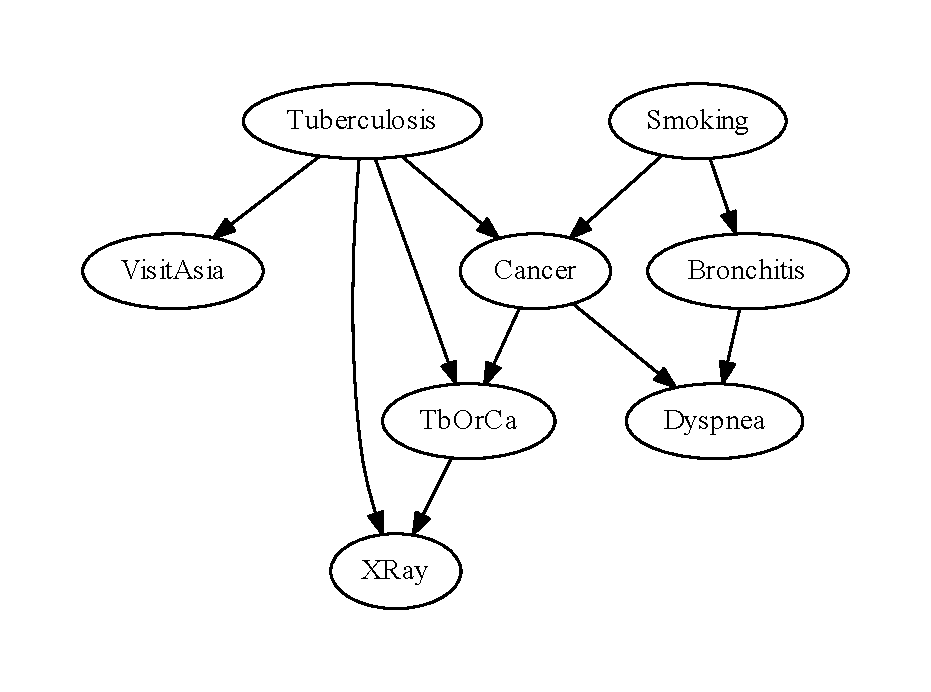
\includegraphics[scale=0.5]{asia_genie_1000_bayesian_search.pdf}  
    \caption{}
  \end{subfigure}
  \begin{subfigure}[b]{0.48\textwidth} 
    \centering
    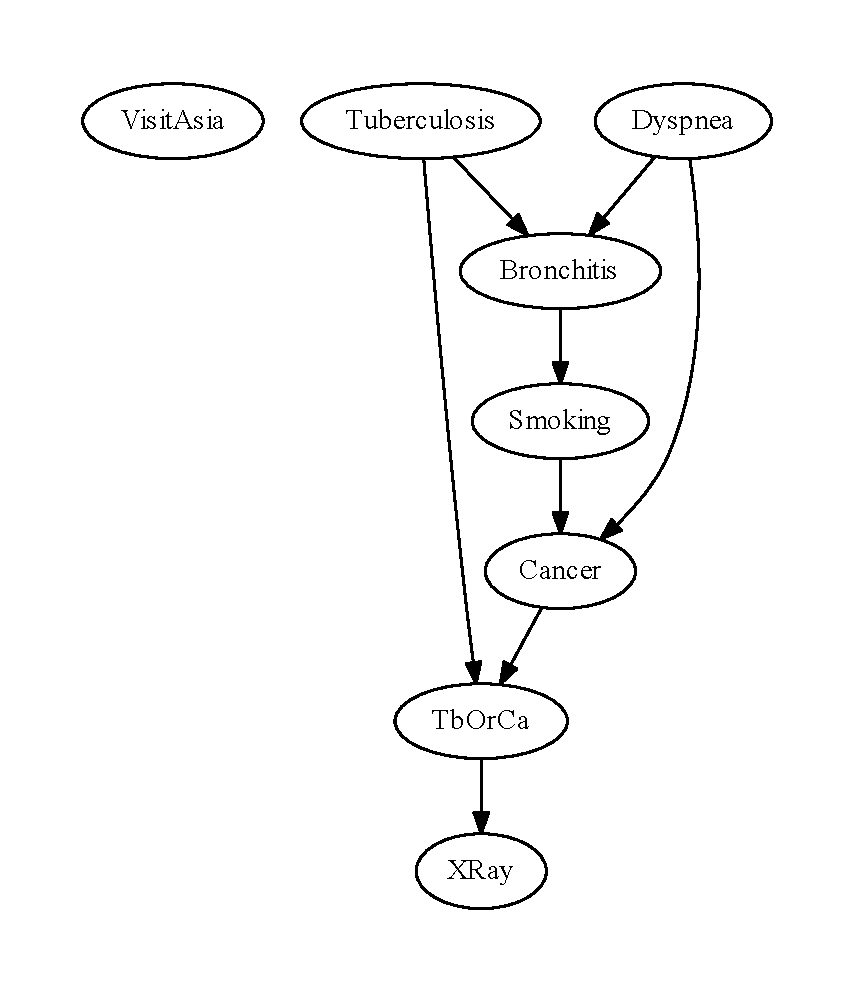
\includegraphics[scale=0.5]{asia_genie_1000_k2.pdf}  
    \caption{}
  \end{subfigure}
  \begin{subfigure}[b]{0.9\textwidth} 
    \centering
    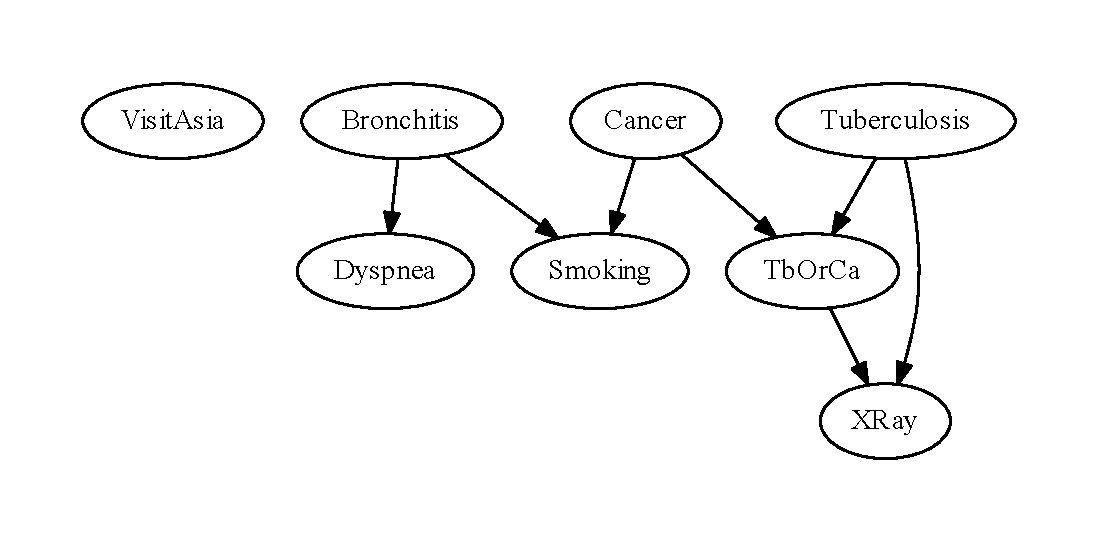
\includegraphics[scale=0.5]{asia_genie_1000_pc.pdf}  
    \caption{}
  \end{subfigure}
  \caption{ Структуры, выведенные по данным с помощью GeNIe: а "--- алгоритм Bayesian Search;
            б "--- алгоритм K2;
            в "--- алгоритм PC;}
  \label{fig:domain:programs:genie_infered_structrures}
\end{figure}


\begin{figure}[ht]
\centering
  \begin{subfigure}[b]{0.49\textwidth} 
    \centering
    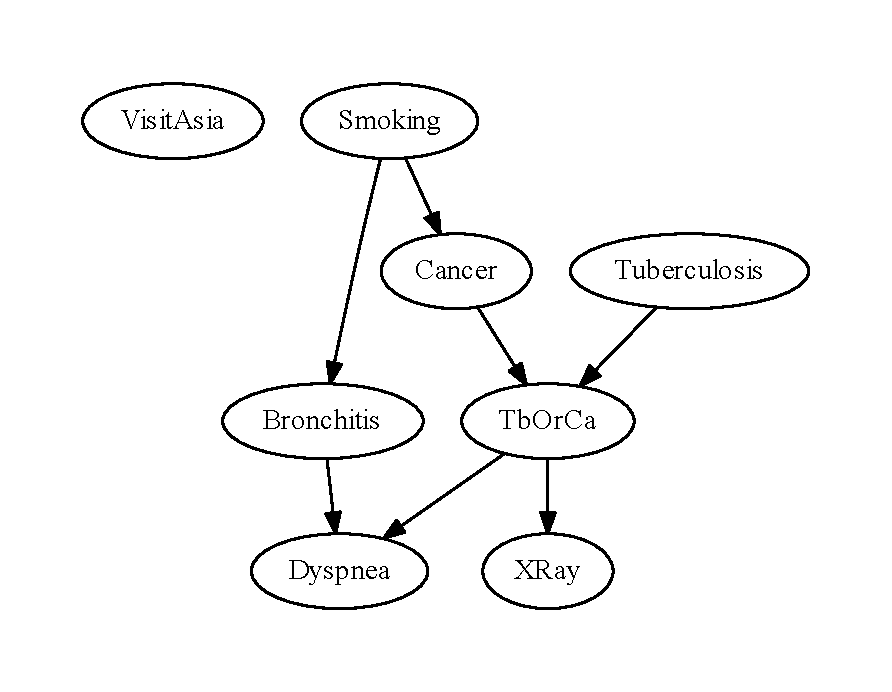
\includegraphics[scale=0.45]{asia-learned-by-terent-random-1000.pdf}  
    \caption{}
  \end{subfigure}
  \begin{subfigure}[b]{0.48\textwidth} 
    \centering
    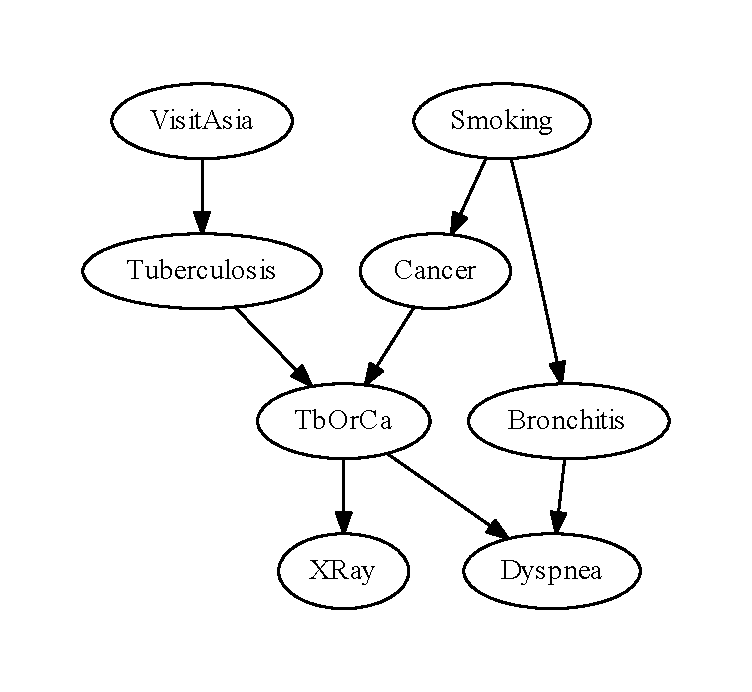
\includegraphics[scale=0.45]{asia_reference_net.pdf}  
    \caption{}
  \end{subfigure}

  \caption{ Выведенная из данных и оригинальная сеть Asia: а "--- алгоритм из разработанной библиотеки, использующий оценку МДО;
            б "--- истинная сеть Asia}
  \label{fig:domain:programs:our_impl_plus_asia}
\end{figure}